\documentclass{standalone}

\usepackage[english]{babel}
\usepackage[linesnumbered, ruled, vlined]{algorithm2e}

\usepackage{caption}

% to create listings

\usepackage{listings, lstautogobble}
\lstset{
  autogobble=true,
  frame=single,
}

\lstdefinelanguage{coq}[Objective]{Caml}{
  morekeywords={Structure, Definition, Inductive, list, return},
  sensitive=true
}

% to frame text

\usepackage{framed}

% to define font size

\usepackage{ulem}
\usepackage{moresize}
\usepackage{anyfontsize}

% to use tikz and its libraries

\usepackage{tikz-timing}
\usepackage{tikz}

\usetikzlibrary{backgrounds}
\usetikzlibrary{positioning, calc, arrows, shapes, automata, petri, patterns}

% to use tikzmark, to place and refer to marks outside the current figure

\tikzset{every picture/.style={remember picture}}

% styles for transitions

\tikzset{transition/.append style={fill=black!20, thick}}
\tikzset{transition/.append style={fill=black!20, thick}}

% styles for test and inhib arcs.

\tikzstyle{test}=[pre, *-]
\tikzstyle{inhib}=[pre, o-]

% to use colors

\usepackage{xcolor}

%%%%%%%%%%%%%%%%%%%%%%%%%%%%%%%%%%%%%%%%%%%%%%%%%%
%                  BEGIN DOCUMENT                %
%%%%%%%%%%%%%%%%%%%%%%%%%%%%%%%%%%%%%%%%%%%%%%%%%%

\begin{document}

\begin{minipage}{0.26\textwidth}
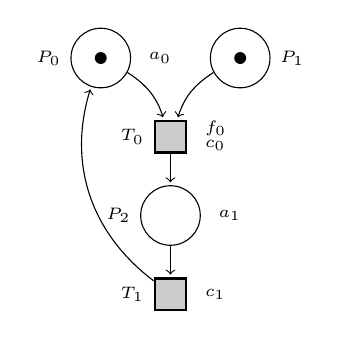
\begin{tikzpicture}
  \node[place, tokens=1] (p0) [label={left:\ssmall $P_0$}] {};
  \node[right =3pt of p0] {\ssmall $a_0$};
  
  \node[place, tokens=1] (p1) [right =of p0, label={right:\ssmall $P_1$}] {};
  \node[place] (p2) at ($(p0)!0.5!(p1)-(0, 2)$) [label={left:\ssmall $P_2$}] {};
  \node[right =3pt of p2] {\ssmall $a_1$};
  
  \node[transition] (t0) at ($(p0)!0.5!(p1)-(0, 1)$) [label={left:\ssmall $T_0$}] {}
  edge[pre, bend right=20] (p0)
  edge[pre, bend left=20] (p1)
  edge[post] (p2);
  
  \node[right =3pt of t0, yshift=+3pt] {\ssmall $f_0$};
  \node[right =3pt of t0, yshift=-3pt] {\ssmall $c_0$};
  
  \node[transition] (t1) at ($(p2)-(0, 1)$) [label={left:\ssmall $T_1$}] {}
  edge[pre] (p2)
  edge[post, bend left=35] (p0);
  
  \node[right =3pt of t1] {\ssmall $c_1$};  
\end{tikzpicture}
\end{minipage}\hspace{1pt}
\begin{minipage}{0.36\textwidth}
  \begin{framed}
    \fontsize{8}{9}\selectfont
    $c_0$: $heat\_sensor\_value\ > 10$\\
    $f_0$: $x := 1;\ y := 0;$\\
    $c_1$: $x\ \&\&\ y;$
    \par
  \end{framed}
\end{minipage}

\end{document}
%%% Local Variables:
%%% mode: latex
%%% TeX-master: t
%%% End:
